\chapter{Post-Quantum Security for Edge AI Pipelines}
\label{ch:edge-ai}

Chapter~\ref{ch:dpu-pqc} evaluated post-quantum primitives in isolation, where a KEM or a signature is the only workload on the processor. Real deployments are rarely so tidy. In an edge artificial-intelligence system the cryptography is one stage in a longer, latency-critical pipeline, sharing processors, memory bandwidth, and trust boundaries with the very workload it protects. This chapter re-examines the offload question inside such a pipeline, taking real-time image inference as its testbed.

\section{Securing the Edge AI Data Path}
\label{sec:edge-datapath}

An edge-AI inference pipeline turns a stream of raw sensor frames into decisions in real time. Each frame traverses a sequence of stages: it is received from the network, decoded from its wire format (JPEG, TIFF, or raw), preprocessed---color-space converted, resized, and normalized---into a tensor, and finally consumed by a neural network on a GPU. The pipeline runs against a hard, recurring deadline: at 30~frames per second the entire per-frame sequence must complete within roughly 33~milliseconds, or frames are dropped and the system falls behind the physical process it observes.

Adding post-quantum protection inserts new mandatory work into this path. Before a frame can be trusted, its authenticity must be verified and its contents decrypted---and these steps now sit on the critical path of every frame, inside the same 33~ms budget. The question is not merely whether the cryptography is fast in isolation, which Chapter~\ref{ch:dpu-pqc} already addressed, but where it can run without starving the stages around it.

The conventional placements are both unsatisfactory. Performing authentication and decryption on the host CPU consumes general-purpose cycles and, more importantly, leaves decrypted frames and key material resident in the host's memory---inside the host trust domain, where a compromised operating system or hypervisor can observe them. Performing the cryptographic and preprocessing work on the GPU instead steals streaming-multiprocessor (SM) capacity from the inference model that the GPU was provisioned to run, and still routes plaintext through the host on its way to the device. Neither option both preserves the frame budget and keeps plaintext out of the host trust domain, which is precisely the gap this chapter's contribution addresses.

\section{Motivating Domains and Threat Scenarios}
\label{sec:edge-threats}

The edge-AI pattern recurs across domains where the sensor feed is both sensitive and safety-relevant. Smart-camera surveillance and access control turn video into identity and intrusion decisions; medical imaging pipelines feed diagnostic models from cameras and scanners; industrial and autonomous systems drive actuators from vision in closed control loops. In each case the frames carry private or regulated content, and the decisions they drive have physical consequences.

This dual sensitivity defines the threat model. Confidentiality is the obvious concern---an eavesdropper on the sensor link, or a compromised host, must not recover the raw imagery---and it motivates encryption of the frame stream. But integrity and freshness matter just as much: an adversary who can inject, replay, or tamper with frames can steer the model's output, blinding a surveillance system or spoofing an industrial controller, without ever breaking confidentiality. Defending against this requires that every frame be \emph{authenticated}, not merely decrypted, and that stale or replayed frames be rejected. Post-quantum authentication is therefore a first-class requirement of the pipeline rather than an optional add-on, and it must be delivered within the same real-time budget as the frames themselves.

\section{How KEMs Bootstrap the Data Plane}
\label{sec:edge-kem-bootstrap}

Protecting a high-rate frame stream does not mean running a post-quantum operation on every frame. The asymmetric primitives of Chapter~\ref{ch:dpu-pqc} are comparatively expensive and are used sparingly, to \emph{bootstrap} the data plane rather than to carry it. At session setup, a post-quantum KEM (ML-KEM) establishes a shared symmetric secret between the sensor endpoint and the receiver, exactly as sketched in Figure~\ref{fig:kem-flow}; a post-quantum signature (ML-DSA) authenticates that exchange so the receiver knows the key was negotiated with the genuine peer. This handshake runs once per session.

From that point on, the shared secret keys a symmetric authenticated-encryption-with-associated-data (AEAD) cipher---AES-GCM---which protects the bulk frame stream. Symmetric AEAD supplies confidentiality, per-frame integrity, and, through sequence numbering, the freshness that defeats replay, all at a per-frame cost orders of magnitude below an asymmetric operation. The division of labor is thus clean: the post-quantum KEM and signature amortize their cost across the whole session, while the per-frame data plane runs on fast symmetric cryptography. This separation is what makes post-quantum protection compatible with a 30~fps deadline in the first place, and it locates the real-time challenge not in the post-quantum arithmetic itself---whose internals are treated in Section~\ref{sec:pqc-families}---but in sustaining the symmetric decrypt-and-authenticate stage frame after frame, alongside decoding and preprocessing, without missing the budget.

\section{Terminating Frames at Network Ingress}
\label{sec:edge-terminate}

The architecture evaluated in this chapter resolves the placement dilemma of Section~\ref{sec:edge-datapath} by terminating frames at network ingress, on the DPU, before they ever reach the host. As each frame arrives, the DPU's general-purpose Arm cores authenticate it, decrypt it, and perform the image decoding and preprocessing, assembling an inference-ready tensor. Only that tensor is then transferred to the GPU for inference. Figure~\ref{fig:edge-ai-pipeline} contrasts this DPU-terminated path with the conventional host- and GPU-centric paths.

\begin{figure}[htbp]
  \centering
  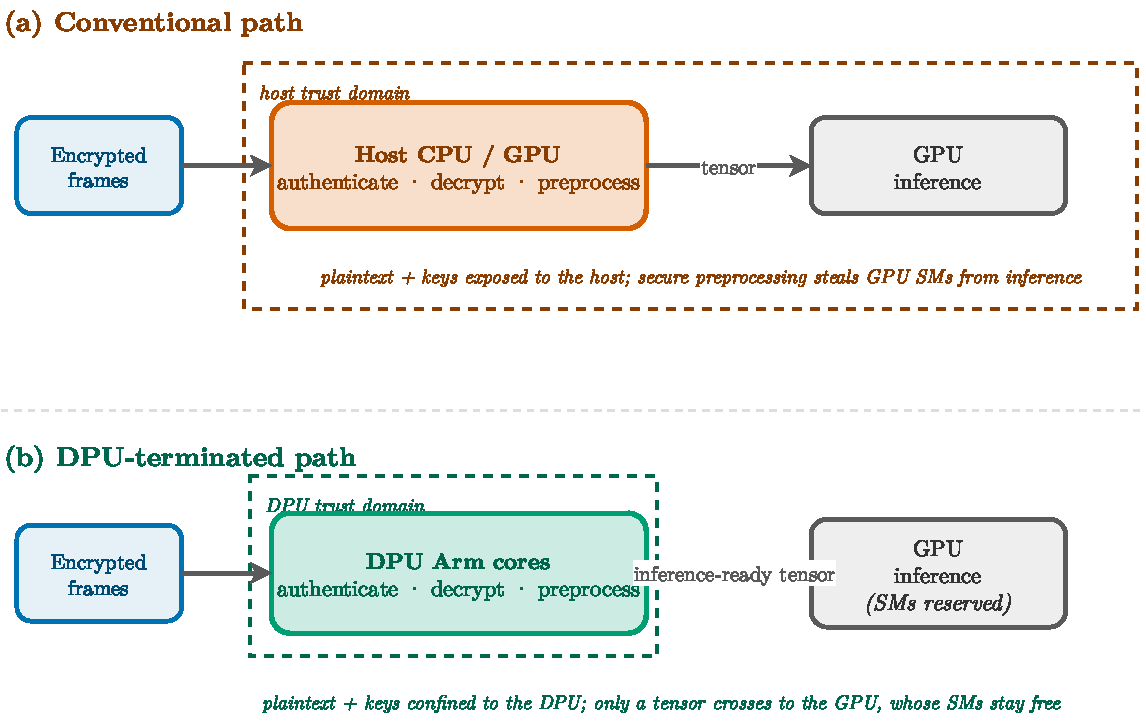
\includegraphics[width=\linewidth]{figures/chapter6/edge_ai_pipeline.pdf}
  \caption{Two ways to place the secure preprocessing of an edge-AI frame
  stream. In the \textbf{conventional path} (top), encrypted frames enter the
  host, which authenticates, decrypts, and preprocesses them---leaving plaintext
  and key material in the host trust domain---or offloads that work to the GPU,
  stealing streaming-multiprocessor (SM) capacity from the inference model. In
  the \textbf{DPU-terminated path} (bottom), frames are authenticated,
  decrypted, and preprocessed on the DPU's Arm cores at network ingress; only an
  inference-ready tensor crosses into the GPU. Plaintext and keys never enter the
  host trust domain, and the GPU's SMs are reserved entirely for inference.}
  \label{fig:edge-ai-pipeline}
\end{figure}

This placement delivers two benefits at once. It preserves the GPU's SMs for the inference model, since the decode, decrypt, and preprocess stages no longer compete for them; and it confines plaintext frames and key material to the DPU, isolating them from the host trust domain and shrinking the attack surface to the network device itself. The design thus turns the DPU from a mere offload target into a security boundary---the same architectural move made for QKD key material in Chapter~\ref{ch:qkd-dpu}, now applied to an application data plane.

\section{Contribution and Articles}
\label{sec:edge-context}

This chapter is built around one contribution (P6), \enquote{Real-Time Post-Quantum Secured Image Pipeline on NVIDIA BlueField-3 DPU}, which realizes and evaluates the DPU-terminated architecture of Section~\ref{sec:edge-terminate} on real hardware, addressing \textbf{RQ1} at the level of a complete application pipeline.

This manuscript is under review at the IEEE International Conference on Algorithms and Architectures for Parallel Processing (ICA3PP). The paper implements a real-time, post-quantum-secured image pipeline on an NVIDIA BlueField-3 DPU, offloading both image I/O and the cryptographic stages---ML-KEM key establishment and ML-DSA authentication bootstrapping a symmetric per-frame data plane---from the host onto the DPU's Arm cores, and delivering an inference-ready tensor to the GPU. Its headline results establish that the approach is not merely secure but real-time: on a single Arm core the secure receive path sustains 1080p video at 85~frames per second for JPEG and 98~frames per second for TIFF, and the per-frame post-quantum stage consumes only 23\% of the 30~fps budget for a raw 1080p payload. Post-quantum protection, in other words, fits comfortably within a real-time edge-AI pipeline when the work is placed on the DPU.

Read against Chapter~\ref{ch:dpu-pqc}, this contribution completes Part~\ref{part:pqc}'s argument. The isolated-primitive studies showed \emph{that} post-quantum cryptography can be offloaded efficiently; the pipeline study shows that the offload advantage---GPU capacity preserved, host trust domain kept clear, deadline met---survives contact with a full, contention-prone application workload.

\includedpaper{P6}{Real-Time Post-Quantum Secured Image Pipeline on NVIDIA BlueField-3 DPU}{meyer2026edgeai}{source-materials/papers/camera-ready/EDGEAI.pdf}

\section{Discussion and Transition}
\label{sec:edge-discussion}

Evaluating post-quantum cryptography inside a live pipeline changes the interpretation of the isolated benchmarks of Chapter~\ref{ch:dpu-pqc}. A primitive's standalone latency is necessary but not sufficient; what ultimately matters is whether the secured pipeline holds its deadline while sharing hardware with decoding, preprocessing, and inference. The DPU-terminated design succeeds precisely because it treats security and the application as a single co-designed data path rather than as layers stacked on a host. Open questions remain---how the approach scales to many concurrent streams and higher resolutions, and how the Arm-core budget is best divided among decode, crypto, and preprocessing under heavier load---but the central claim holds: post-quantum protection can be made real-time at the edge by moving it into the network device.

Both chapters of Part~\ref{part:pqc} have so far treated the DPU as a cooperative and trustworthy substrate---an accelerator that faithfully executes the cryptography and pipelines placed on it. Part~\ref{part:infra} steps back to interrogate that assumption. It examines the programmable datacenter fabric on which these mechanisms ultimately run, and the cross-layer risks that emerge when the network beneath a secure workload does not behave as its designers assumed. The next chapter begins this shift by turning to remote direct memory access over high-throughput optical fabrics, where ordering and timing assumptions that hold in principle can be violated in practice, as taken up in Chapter~\ref{ch:rdma}.
